\chapter{Introduction}

In computer aided geometric design, polynomials are usually expressed in
Bernstein form. Polynomials in this form are usually evaluated by the
de Casteljau algorithm. This algorithm has a round-off error bound
which grows only linearly with degree, even though the number of
arithmetic operations grows quadratically. The Bernstein basis is
optimally suited (\cite{Farouki1987, Delgado2015, Mainar2005})
for polynomial evaluation; it is
typically more accurate than the monomial basis, for example in
Figure~\ref{fig:horner-inferior} evaluation via Horner's method produces
a jagged curve for points near a triple root, but the de Casteljau algorithm
produces a smooth curve. Nevertheless the de Casteljau
algorithm returns results arbitrarily less accurate than the working
precision \(\mach\) when evaluating \(p(s)\) is ill-conditioned.
The relative accuracy of the computed
evaluation with the de Casteljau algorithm (\texttt{DeCasteljau}) satisfies
(\cite{Mainar1999}) the following a priori bound:
\begin{equation}\label{de-casteljau-error}
  \frac{\left|p(s) - \mathtt{DeCasteljau}(p, s)\right|}{\left|p(s)\right|} \leq
  \cond{p, s} \times \bigO{\mach}.
\end{equation}
In the right-hand side of this inequality, \(\mach\) is the computing
precision and the condition number \(\cond{p, s} \geq 1\) only depends
on \(s\) and the Bernstein coefficients of \(p\) --- its expression will
be given further.

\begin{figure}
  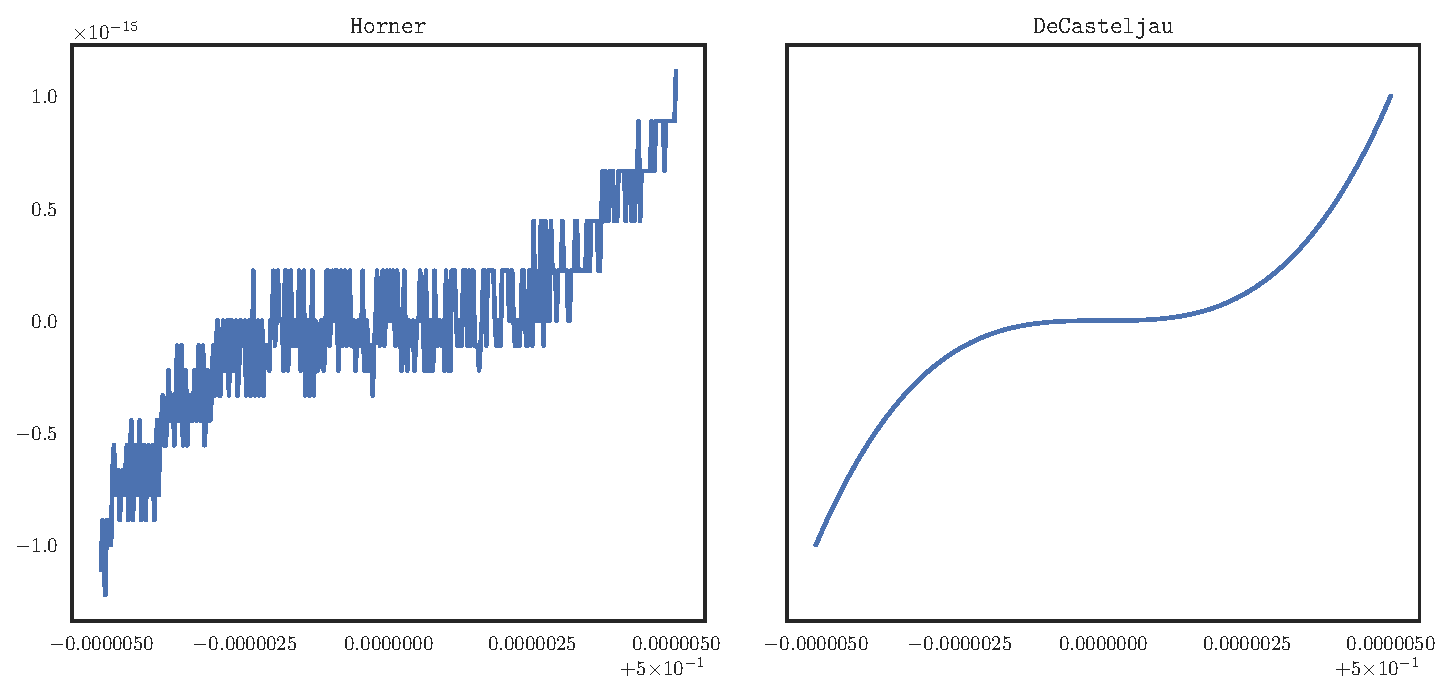
\includegraphics[width=0.9375\textwidth]{../images/chapter1/horner_inferior.pdf}
  \centering
  \captionsetup{width=.75\linewidth}
  \caption{Comparing Horner's method to the de Casteljau method for
    evaluating \(p(s) = (2s - 1)^3\) in the neighborhood of its
    multiple root \(1/2\).}
  \label{fig:horner-inferior}
\end{figure}

For ill-conditioned problems, such as evaluating \(p(s)\) near a
multiple root, the condition number may be arbitrarily large, i.e.
\(\cond{p, s} > 1 / \mach\), in
which case most or all of the computed digits will be incorrect.
In some cases, even the order of magnitude of the computed value
of \(p(s)\) can be incorrect.

To address ill-conditioned problems, error-free transformations (EFT) can
be applied in \textit{compensated algorithms} to account for round-off.
Error-free transformations were studied in great detail in \cite{Ogita2005}
and open a large number of applications.
In \cite{langlois_et_al:DSP:2006:442}, a compensated Horner's algorithm was
described to evaluate a polynomial in the monomial basis. In \cite{Jiang2010},
a similar method was described to perform a compensated version of the de
Casteljau algorithm. In both cases, the \(\cond{p, s}\) factor is moved
from \(\mach\) to \(\mach^2\) and the computed value is as accurate
as if the computations were done in twice the working precision. For example,
the compensated de Casteljau algorithm (\texttt{CompDeCasteljau}) satisfies
\begin{equation}\label{de-casteljau-2-error}
  \frac{\left|p(s) - \mathtt{CompDeCasteljau}(p, s)\right|}{
    \left|p(s)\right|} \leq \mach + \cond{p, s} \times
    \bigO{\mach^2}.
\end{equation}
For problems with \(\cond{p, s} < 1 / \mach^2\), the relative error
is \(\mach\), i.e. accurate to full precision, aside from rounding to the
nearest floating point number. Figure~\ref{fig:jlcs-10} shows this shift
in relative error from \texttt{DeCasteljau} to \texttt{CompDeCasteljau}.

\begin{figure}
  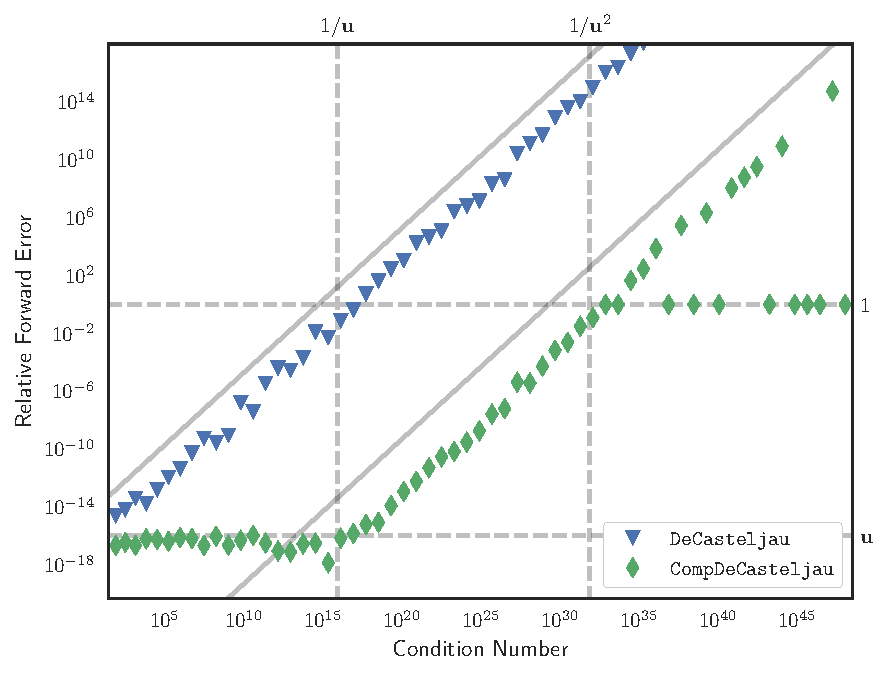
\includegraphics[width=0.8125\textwidth]{../images/chapter1/jlcs10_plot.pdf}
  \centering
  \captionsetup{width=.75\linewidth}
  \caption{Evaluation of \(p(s) = (s - 1)\left(s - 3/4\right)^7\)
    represented in Bernstein form.}
  \label{fig:jlcs-10}
\end{figure}

In \cite{Graillat2009}, the authors generalized the compensated Horner's
algorithm to produce a method for evaluating a polynomial as if
the computations were done in \(K\) times the working precision for
any \(K \geq 2\). This result motivates this paper, though the
approach there is somewhat different than ours. They perform each computation
with error-free transformations and interpret the errors as coefficients of new
polynomials. They then evaluate the error polynomials, which (recursively)
generate second order error polynomials and so on. This recursive property
causes the number of operations to grow exponentially in \(K\). Here, we
instead have a fixed number of error groups, each corresponding to round-off
from the group above it. For example, when
\((1 - s) b_j^{(n)} + s b_{j + 1}^{(n)}\) is computed in floating point, any
error is filtered down to the error group below it.

As in~\eqref{de-casteljau-error}, the accuracy of the compensated
result~\eqref{de-casteljau-2-error} may be arbitrarily bad for ill-conditioned
polynomial evaluations. For example, as the condition number grows in
Figure~\ref{fig:jlcs-10}, some points have relative error exactly equal to
\(1\); this indicates that \(\mathtt{CompDeCasteljau}(p, s) = 0\), which is
a complete failure to evaluate the order of magnitude of \(p(s)\). For
root-finding problems \(\mathtt{CompDeCasteljau}(p, s) = 0\) when
\(p(s) \neq 0\) can cause premature convergence and incorrect results.
We describe how to defer rounding into progressively
smaller error groups and improve the accuracy of the computed result by a
factor of \(\mach\) for every error group added. So we derive
\texttt{CompDeCasteljauK}, a \(K\)-fold compensated de Casteljau algorithm
that satisfies the following a priori bound for any arbitrary integer \(K\):
\begin{equation}
  \frac{\left|p(s) - \mathtt{CompDeCasteljauK}(p, s, K)\right|}{
    \left|p(s)\right|} \leq \mach + \cond{p, s} \times
    \bigO{\mach^K}.
\end{equation}
This means that the computed value with \texttt{CompDeCasteljauK} is now
as accurate as the result of the de Casteljau algorithm performed in
\(K\) times the working precision with a final rounding back to the
working precision.

The paper is organized as follows. Section~\ref{sec:notation} establishes
notation for error analysis with floating point operations, reviews
results about error-free transformations and reviews the
de Casteljau algorithm. In Section~\ref{sec:compensated-2},
the compensated algorithm for polynomial evaluation from \cite{Jiang2010} is
reviewed and notation is established for the expansion. In
Section~\ref{sec:compensated-k}, the \(K\)-compensated algorithm is provided
and a forward error analysis is performed. Finally, in
Section~\ref{sec:numerical} we perform two numerical experiments to
give practical examples of the theoretical error bounds.
